\section{Konzept (Joshua Hörmann)}
In diesem Kapitel wird ein Überblick über das Architekturkonzept gegeben und das Datenbankmodell erklärt.
\subsection{Architekturkonzept}
\begin{figure}[H]
	\centerline{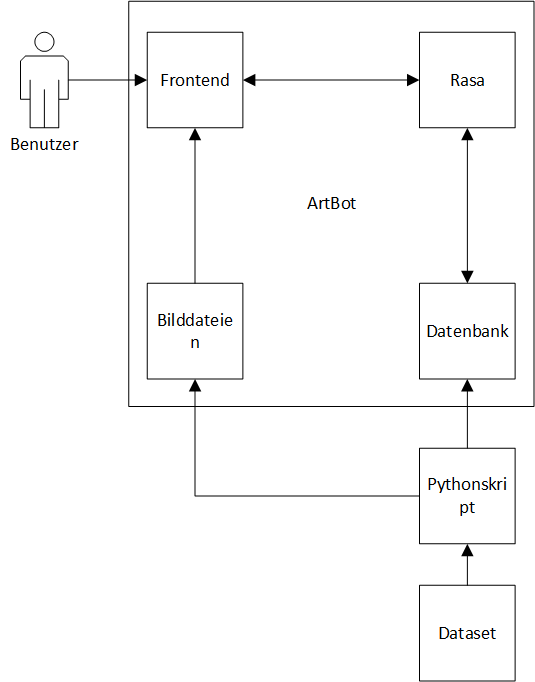
\includegraphics[width=0.6\linewidth]{figures/konzept.png}}
	\caption{Architekturkonzept des ArtBots}
	\label{konzept}
\end{figure}

In Abbildung \ref{konzept} ist das Konzept des ArtBots dargestellt. Dabei interagiert der Benutzer mit einem Frontend, welches mit Rasa verbunden ist und die eingegebenen Befehle an Rasa weitergibt. Rasa bearbeitet diese entweder intern oder stellt eine Anfrage an die Datenbank. Die entsprechende Antwort wird an das Frontend zurückgegeben und dort ausgegeben. Wenn ein Bild zur Ausgabe benötigt wird, holt sich das Frontend die entsprechende Bilddatei über den Dateinamen. Die Datenbank sowie der Ordner mit den Bilddateien werden mithilfe eines Python-Skripts mit Daten aus dem Dataset befüllt. Der Aufbau der fertigen Implementierung ist unter \ref{umsetzung} dargestellt. Im Folgendem wird das Datenbankmodell vorgestellt.

\subsection{Datenbankmodell}\label{datenbankmodell}
Der Aufbau der Datenbank ist simpel gehalten, da wir nur eine vereinfachte Abbildung des Datensatzes benötigt haben. Daher enthält er nur die beiden Tabellen Artists und Pictures. Die Tabelle Artists enthält die Künstler mit ihrem Namen als Primary Key und dem Geburtsdatum als zusätzliches Attribut. Das Geburtsdatum wird noch nicht verwendet, wir haben es aber für die spätere Erweiterbarkeit eingefügt. Die Tabelle Pictures enthält die Eckdaten der einzelnen Bilder. Dabei sind der Dateiname, der Name des Künstlers, der Titel, die Epoche, sowie das Genre abgelegt. Der Filename ist dabei der Primary Key und der Künstlername ein Foreign Key. Dieser Aufbau ist in \ref{datenbank} illustriert. Zuerst hatten wir noch versucht die Bilder ebenfalls in der Datenbank abzulegen, aber da die Datenbank dadurch viel zu groß wurde und es zu Konvertierungsschwierigkeiten beim Einfügen und Auslesen aus der Datenbank kam, haben wir uns gegen diesen Ansatz entschieden. Die Bilder haben wir daraufhin in einen extra Bilderordner abgelegt.

\begin{figure}[H]
	\centerline{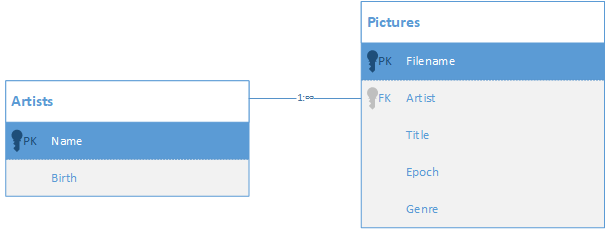
\includegraphics[width=0.7\linewidth]{figures/Datenbankmodell.png}}
	\caption{Darstellung des Datenbankmodells}
	\label{datenbank}
\end{figure}

\newpage

